%%%%%%%%%%%%%%%%%%%%%%%%%%%%%%%%%%%%%%%%%
% Masters/Doctoral Thesis 
% LaTeX Template
% Version 2.4 (22/11/16)
%
% This template has been downloaded from:
% http://www.LaTeXTemplates.com
%
% Version 2.x major modifications by:
% Vel (vel@latextemplates.com)
%
% This template is based on a template by:
% Steve Gunn (http://users.ecs.soton.ac.uk/srg/softwaretools/document/templates/)
% Sunil Patel (http://www.sunilpatel.co.uk/thesis-template/)
%
% Template license:
% CC BY-NC-SA 3.0 (http://creativecommons.org/licenses/by-nc-sa/3.0/)
%
%%%%%%%%%%%%%%%%%%%%%%%%%%%%%%%%%%%%%%%%%

%----------------------------------------------------------------------------------------
%	PACKAGES AND OTHER DOCUMENT CONFIGURATIONS
%----------------------------------------------------------------------------------------

\documentclass[
11pt, % The default document font size, options: 10pt, 11pt, 12pt
%oneside, % Two side (alternating margins) for binding by default, uncomment to switch to one side
english, % ngerman for German
singlespacing, % Single line spacing, alternatives: onehalfspacing or doublespacing
%draft, % Uncomment to enable draft mode (no pictures, no links, overfull hboxes indicated)
%nolistspacing, % If the document is onehalfspacing or doublespacing, uncomment this to set spacing in lists to single
%liststotoc, % Uncomment to add the list of figures/tables/etc to the table of contents
%toctotoc, % Uncomment to add the main table of contents to the table of contents
%parskip, % Uncomment to add space between paragraphs
%nohyperref, % Uncomment to not load the hyperref package
headsepline, % Uncomment to get a line under the header
%chapterinoneline, % Uncomment to place the chapter title next to the number on one line
%consistentlayout, % Uncomment to change the layout of the declaration, abstract and acknowledgements pages to match the default layout
]{MastersDoctoralThesis} % The class file specifying the document structure
\usepackage{scrextend}
\deffootnote[2em]{2em}{2em}{\textsuperscript{\thefootnotemark}\,}
\usepackage[utf8]{inputenc} % Required for inputting international characters
\usepackage[T1]{fontenc} % Output font encoding for international characters
\usepackage{tocloft}
\usepackage{caption}
\usepackage{subcaption}
\usepackage{minted}
\usepackage{pdfpages}
\usepackage{caption}
\usepackage{palatino} % Use the Palatino font by default
\usepackage{etoolbox}
\usepackage{lscape}
\usepackage{multicol,multirow}
 \usepackage{cancel}
 \usepackage{colortbl}
 \usepackage{float}
     \usepackage{amsmath}
          \usepackage[linesnumbered,ruled]{algorithm2e}
\usepackage{listings}
\usepackage{xcolor}
\lstset{language=C++,
	basicstyle=\ttfamily,
	keywordstyle=\color{blue}\ttfamily,
	stringstyle=\color{red}\ttfamily,
	commentstyle=\color{orange}\ttfamily,
	morecomment=[l][\color{magenta}]{\#}
}


% Rotating table
\usepackage{rotating}
\AfterEndEnvironment{myenv}{\restoregeometry}
\newenvironment{myenv}{%
  \newgeometry{top = 0in}%
}{%
  \newpage%
}
\usepackage[font=small,labelfont=bf]{caption} % Required for specifying captions to tables and figures
 \usepackage{pgfgantt}
\usepackage[backend=bibtex,style=authoryear,natbib=true]{biblatex} % Use the bibtex backend with the authoryear citation style (which resembles APA)
\addbibresource{example.bib} % The filename of the bibliography
\definecolor{bleu}{RGB}{37,104,162}
\usepackage[autostyle=true]{csquotes} % Required to generate language-dependent quotes in the bibliography
\renewcommand{\baselinestretch}{1.5}
%----------------------------------------------------------------------------------------
%	MARGIN SETTINGS
%----------------------------------------------------------------------------------------
\geometry{
	paper=a4paper, % Change to letterpaper for US letter
	inner=2cm, % Inner margin
	outer=3cm, % Outer margin
	bindingoffset=.5cm, % Binding offset
	top=1cm, % Top margin
	bottom=1.3cm, % Bottom margin
	%showframe, % Uncomment to show how the type block is set on the page
}

%----------------------------------------------------------------------------------------
%	THESIS INFORMATION
%----------------------------------------------------------------------------------------

\thesistitle{\textcolor{bleu}{Genomic Data Processing} \linebreak \newline
\normalsize{Hardware Implementation of an Indexed Sequence Mapper}} % Your thesis title, this is used in the title and abstract, print it elsewhere with \ttitle
\supervisor{\textcolor{bleu}{Prof. Yann \textsc{Thoma}}} % Your supervisor's name, this is used in the title page, print it elsewhere with \supname
\examiner{} % Your examiner's name, this is not currently used anywhere in the template, print it elsewhere with \examname
\degree{Bachelor in Computer Science} % Your degree name, this is used in the title page and abstract, print it elsewhere with \degreename
\author{\textcolor{bleu}{Arthur \textsc{Passuello}}} % Your name, this is used in the title page and abstract, print it elsewhere with \authorname
\addresses{} % Your address, this is not currently used anywhere in the template, print it elsewhere with \addressname

\subject{} % Your subject area, this is not currently used anywhere in the template, print it elsewhere with \subjectname
\keywords{} % Keywords for your thesis, this is not currently used anywhere in the template, print it elsewhere with \keywordnames
\university{\href{http://www.university.com}{HEIG-VD}} % Your university's name and URL, this is used in the title page and abstract, print it elsewhere with \univname
\department{\href{http://department.university.com}{\textcolor{bleu}{ } }} % Your department's name and URL, this is used in the title page and abstract, print it elsewhere with \deptname
\group{\href{http://researchgroup.university.com}{\textcolor{bleu}{ }}} % Your research group's name and URL, this is used in the title page, print it elsewhere with \groupname
\faculty{\href{http://unil.ch}{\textcolor{bleu}{Faculté d'Informatique Embarquée}}} % Your faculty's name and URL, this is used in the title page and abstract, print it elsewhere with \facname
\setcounter{chapter}{-1}
\AtBeginDocument{
\hypersetup{pdftitle=\ttitle} % Set the PDF's title to your title
\hypersetup{pdfauthor=\authorname} % Set the PDF's author to your name
\hypersetup{pdfkeywords=\keywordnames} % Set the PDF's keywords to your keywords
\hypersetup{allcolors=black}
}
\setcounter{tocdepth}{0}
\setcounter{tocdepth}{5} %shows all levels incl. paragraph
\begin{document}

\frontmatter % Use roman page numbering style (i, ii, iii, iv...) for the pre-content pages

\pagestyle{plain} % Default to the plain heading style until the thesis style is called for the body content

%----------------------------------------------------------------------------------------
%	TITLE PAGE
%----------------------------------------------------------------------------------------

\begin{titlepage}

\vspace*{-20mm}
\includegraphics[scale = 0.5]{Figures/heigvd_logo.png}
\begin{center}
\textsc{\Large Bachelor Thesis}\\[0.5cm] % Thesis type

\HRule \\[0.4cm] % Horizontal line
{\huge \bfseries \ttitle\par}\vspace{0.4cm} % Thesis title
\HRule \\[1.5cm] % Horizontal line
\begin{minipage}[t]{0.4\textwidth}
\begin{flushleft} \large
\emph{Autor:}\\
\href{http://www.johnsmith.com}{\authorname} % Author name - remove the \href bracket to remove the link
\end{flushleft}
\end{minipage}
\begin{minipage}[t]{0.4\textwidth}
\begin{flushright} \large
\emph{Supervisor:} \\
\href{http://www.jamessmith.com}{\textcolor{red}{\supname}} \linebreak
\textit{\small{HEIG-VD}} \linebreak  % Supervisor name - remove the \href bracket to remove the link

\emph{Expert:} \\
\href{http://www.jamessmith.com}{\textcolor{bleu}{????}} \linebreak 
\textit{\small{???????}}
\end{flushright}
\end{minipage}\\[1.5cm]

\large \textit{Presented at the 2018 Autumn session under the supervision \linebreak of Prof. Yann Thoma}\\[0.3cm] % University requirement text
\textit{at the}\\[0.4cm]\textcolor{bleu}{
Faculté d'Informatique Embarquée \\ HEIG-VD}\\[1cm] % Research group name and department name
{\large \today}\\ % Date
%\includegraphics{Logo} % University/department logo - uncomment to place it
\vfill
\end{center}
\end{titlepage}

%----------------------------------------------------------------------------------------
%	QUOTATION PAGE
%----------------------------------------------------------------------------------------
\thispagestyle{empty}
\newpage

\vspace*{0.2\textheight}


\begin{figure*}[h]
	\centering

	\includegraphics[scale = 0.6]{Figures/xkcd.png}
		\captionsetup{labelformat=empty}% redefines the caption setup of the figures environment in the beamer class.
	\caption{DNA}
	\label{XKCD}
\end{figure*}

\noindent\enquote{ Relevant xkcd.\footnote{source : \textit{\href{https://xkcd.com/1605/}{https://xkcd.com/1605/}}}}\bigbreak

%----------------------------------------------------------------------------------------
%	ABSTRACT PAGE
%----------------------------------------------------------------------------------------

\begin{abstract}
\addchaptertocentry{\abstractname{}} % Add the abstract to the table of contents


\end{abstract}

\begin{extraAbstract}
\addchaptertocentry{Résumé{}} % Add the abstract to the table of contents
BLABLABLA
\end{extraAbstract}
\newpage
\begin{center}
	\Huge
	Glossary
	\normalsize
\end{center}
\hspace*{-10mm}\begin{tabular}{|l|p{5cm}|p{8.5cm}|}
	\hline
\rowcolor{black}\hfill\textcolor{white}{	\textbf{Abréviation}}&\textcolor{white}{\textbf{Terme}}&\textcolor{white}{\textbf{Définition}}\\
	\hline
	HMC & Hybrid Memory Cube & Mémoire constituée de couches empilées de mémoire de type DRAM. \\
	\hline
	BWT & Burrows-Wheeler Transform & Prétraitement des données \href{https://fr.wikipedia.org/wiki/Transform%C3%A9e_de_Burrows-Wheeler}{voir ici} \\
	\hline
	FM-Index & Full-text Minute-size Index  & Principe de compression sans perte, \href{https://fr.wikipedia.org/wiki/FM-index}{Voir ici} \\
\hline
	REDS & Reconfigurable Embedded Digital System & Institut de prestige de l'HEIG \\
\hline
	PEHAGA & Power-Efficient Hardware Acceleration of Genomic Data & ??? \\
	\hline
\end{tabular}
\newpage
%----------------------------------------------------------------------------------------
%	LIST OF CONTENTS/FIGURES/TABLES PAGES
%----------------------------------------------------------------------------------------
\textcolor{bleu}{
\tableofcontents} % Prints the main table of contents

% \listoffigures % Prints the list of figures

% \listoftables % Prints the list of tables

%----------------------------------------------------------------------------------------
%	THESIS CONTENT - CHAPTERS
%----------------------------------------------------------------------------------------
\mainmatter % Begin numeric (1,2,3...) page numbering

\pagestyle{thesis} % Return the page headers back to the "thesis" style
\setcounter{page}{1}
\setcounter{chapter}{0}
\cftsetindents{subsubsection}{0.5in}{0.5in}
% Include the chapters of the thesis as separate files from the Chapters folder
% Uncomment the lines as you write the chapters



% Chapter 1

\chapter{Introduction} % Main chapter title

\label{Chapter1} % For referencing the chapter elsewhere, use \ref{Chapter1} 

%----------------------------------------------------------------------------------------


%----------------------------------------------------------------------------------------
\textit{DNA} sequencing is considered to be a major breakthrough in both medical and biological research. Despite being at first a very lengthy process, the development of new parallel \textit{high-throughput sequencing} (HTS) \footnote{CITE ILLUMINA} technologies allowed very fast and inexpensive sequencing \footnote{CITATION}. Unfortunately, the same breakthrough has not been made with the processing of those data. 
As a matter of fact, the rate at which genomic data is generated exceeds substantially the rate at which it can be processed and this issue might become the next major \textsl{Big Data} issue, surpassing current massive data originator\footnote{http://journals.plos.org/plosbiology/article?id=10.1371/journal.pbio.1002195} .\\

Current DNA sequencing software, such as \textit{Bowtie}\footnote{citer}, use optimal data structures and highly parallelized algorithms in order to reach a maximum processing speed but the whole sequencing still requires several days of computation. Indeed, even though those softwares run on ultra-fast CPUs and pass through highly optimizing compilers, they suffer from various forms of processing overhead due to the heavier, nonspecific environment that are an operating systems and CPUs.

With this in mind, this section will start by providing a further description of genomic data, to then extract from it the main problematic and the research question of this thesis. Finally, the global structure of this document will be introduced through the method introduction.

\section{Genomics \& Genomic Data}

\textit{Genomics} is an area within \textit{Genetics} that focuses on sequencing and analyzing organism's genome (\cite{genomic}). The whole \textit{genome} is contained in every living cell  encoded in \textit{DNA} and, for the human race, distributed over 22 chromosomes, each of which in two copies, and two sex chromosomes. Every DNA sequence consists of combinations of four different nucleo-bases A, C, G and T (respectively \textit{adenine, cytosine, guanine} and \textit{thymine}) in a double-helix form. This shape consists of two complementary strands i.e. both strands contain the same information and one is the \textit{reverse} complement of the other (A always pairs with T, and G with C). The sequence length varies a lot between organisms, from around a million of pairs for bacteria, to hundred of billions for some fish and plants. Typical length for humans is around 3 billions of pairs. \\

Furthermore, the actual sequences contained in a genomes are highly redundant. Those redundancies, serving multiples purpose and due to several causes, make the whole DNA sequence full of superfluous information that significantly further burdens
JE SAIS PAS QUOI DIRE OK

The size of those genomes therefore requires a large amount of processing to acquire, of space to store and most importantly, a huge amount of both to extract useful information from it. The goal of genomic data analysis is to determine the functions of specific genes, their origins and their evolution among many other information. An efficient way to do so is to determine for each species a reference genome which can then be used to as a map. This method allows researcher to identify measured samples as belonging to those references and eventually enables the identification of specific sequences to precise species and biological functions. \\

Finally, the most common used sequencing techniques consists of randomly fragmenting the genome into smaller sequences, only long in the order of the thousands bases, using those to rebuild the whole sequence by mapping them onto a known reference. Although this process allows an easier manipulation of those short sequences, or \textit{reads}, and shows to be much quicker than other reading methods, it presents a major downside. In order to minimize the impact of potential reading errors and to ensure enough read overlap to cover the whole genome (those being random), a certain rate of redundancy in those reads must be reached. In the end, the combined size of such a sequencing is generally expected to be 10 times bigger than the actual DNA, with no concrete guarantee it is really complete. As mentioned, all those ready must then be mapped onto a reference in order to reconstruct the original sequence, this matter is further discussed in the next section and is the main interest of this thesis. 

\section{Problematic}

Genomic data is thus foreseen to become a major \textit{Big Data} issue, its amount increasing at a faster rate than current data processing technologies and despite multiple highly optimized tools designed to increase processing throughput. The current pipeline, cannot seem to catch up. A coarse example of the genomic analysis pipeline is presented below. \\

\begin{minipage}[t]{0.60\textwidth}
\begin{figure}[H]
    \centering
    \includegraphics[scale = 0.4]{Figures/pipeline.png}
    \caption{Will be replaced by a homemade figure}
    \label{fig:analysispipe}
\end{figure}
\end{minipage}
\begin{minipage}[t]{0.350\textwidth}
After being read, usual genome sequencer produce 5 types of symbols, the 4 nucleobases A, C, G, T and another symbol, $N$, present when the sequencer could not determine which base to assign to a read sample. Then comes the alignment, an essential step to any further work on those data. \\

\end{minipage}
\vspace*{5mm}



As an obligatory procedure to any further work on genomic data, increasing the performance on read alignment seems greatly needed. As mentioned earlier, processing those pieces of information means processing a huge volume of rather redundant textual data. This distinctive aspect makes room already for a lot of optimization including data compression and parallel processing and this is where another approach might be pertinent. \\

Hardware accelerators are now a common practice\footnote{CITE} when confronted to a need of performance gain for a specific task in an information system. This approach seems indeed to be very efficient by providing a fully dedicated highly parallelizable system, meaning very little to no processing overhead, for those tasks. In this context, the sequence mapping of a plethora of short reads to one common reference seems like an ideal candidate for such an approach. This idea is the main scope of this project and will be further detailed in the next section.

\section{Research Question}

As mentioned in the previous section beyond the urgent need of quick performance improvement of short read alignment in genomic data processing, there might be a real speedup potential in the use of a hardware accelerator for this part of the analysis pipeline. \\

Benefiting from the redundant nature of DNA and alleviating the burden of its size, the \textsl{FM-Index} is an index base on the \textsl{Burrows-Wheeler Transform} data structure that allows fast substring queries in a compressed text. Enabling a sublinear complexity - with respect to the size of the data - for both query time and storage space, it has shown to provide very good performance results in short-read alignment software. \\

Using this index, a very simple operation-wise substring query algorithm can be defined and would then be a good candidate for a hardware implementation. The main idea is to provide a time and memory efficient solution as an alternative to otherwise entirely software solutions. In a second phase, this project will try to explore the performances of such a model in order to determine a final solution offering a significant speedup.

\section{Method Introduction}

This project will start with a custom software implementation of the FM-Index, in \textsl{C++}, in order to both get a better grasp of the concepts at stake, and provide a communication interface for the future hardware module.

 For this second phase, among many hardware solutions, \textsl{FPGAs} seem like an ideal candidate. Enabling a fully dedicated hardware design and able to interact with memory with significantly less overhead than software.

Using \textsl{Hybrid Memory Cube} to store the reference data and \textsl{PCI Express} bus to communicate with a computer, both of which will be further introduced in an upcoming section, this project will then try to design a simple and low latency FM-Index implementation in \textsl{VHDL}. Then, in a final phase, it will try to explore the parallelization possibilities of this solution in order to make the best out of both \textsl{FPGA} and \textsl{HMC} provided advantages.

The next chapter will further introduce the FM-Index through a simple software implementation. Then, Chapter 3 will propose a first sequencial implementation of this index. Next, Chapter 4 will show this solution integration on a board containing both a FPGA and a HMC. Thereafter, a more efficient parallel implementation will be introduced in Chapter 6, followed by its integration in Chapter 7. Finally, Chapter 8 will offer a retrospective look on this thesis and its limitations.
% Chapter Template

\chapter{FM-Index} % Main chapter title

\label{Chapter2} % Change X to a consecutive number; for referencing this chapter elsewhere, use \ref{ChapterX}

%----------------------------------------------------------------------------------------
%	SECTION 1
%----------------------------------------------------------------------------------------
%\begin{figure*}[h]

%	\vspace*{-60mm}
%	\hspace*{60mm}\includegraphics[scale = 0.3]{Figures/xkcd.png}
%\end{figure*}
%\vspace*{15mm}

With the observations afore stated about the nature and form of the data in the context of genomics, it seems obvious that an appropriate data structure for those, along with an efficient algorithm, might to a serious gain in performance in the short reads alignments. The \textsl{FM-Index} is a lossless compression algorithm based on the \textsl{Burrows-Wheeler Transform} that offers such gains by reorganizing the data in a way that may reduce both memory needs and latency of the mapping process. 

Both those concepts are the subject of the next sections, followed by a \textsl{Python} implementation, which aims to better illustrate the whole read alignment process, and a \textsl{C++} implementation of the same algorithm which will be then used for the hardware implementation.

\section{Theoretical Concepts}

Introduced by \textsl{Michael Burrows} and \textsl{David Wheeler} in 1994, the \textsl{Burrows-Wheeler Transform} (BWT) rearranges the characters of a \textit{string} into sequences of similar characters by a series linear operations. Although it does not reduce the size of the input data, the rearrangement thus obtained gets greatly improved compression results. Furthermore, the easy reversibility of the process substantially facilitate data manipulation employed in sequence alignment, such as finding the original position from the determined one in the transform. This process is further detailed in the next section.

\subsection{Burrows-Wheeler Transform Algorithm \& LF-Mapping}

The transform can be divided in 4 main steps\footcite{BWT0} :
\begin{enumerate}
\item Append a special character (usually represented as a \$), lexicographically smaller than any others, at the end of the input string \textrm{T}.
\item Construct a square matrix $M_T$ with each being another iteration of a left rotating shift applied to the original string.
\item Sort $M_T$ in lexicographical order
\item Get the transformed text output $T^{bwt}$ by selecting the last column of $M_T$ 
\end{enumerate}

\begin{figure}[h]
\centering
\includegraphics[scale=0.65]{Figures/bwt.png}
\caption{Illustration of the \textsl{BWT} applied to the string \textit{acaacg}}
 \label{fig:bwt}
 \end{figure}
The figure \ref{fig:bwt} above illustrates the process of the \textsl{BWT}, it will be shown next what is used in the mapping process, but first let us note the following properties :
\begin{enumerate}
\item the process is revertible as it consists exclusively of linear operations
\item all columns are permutations of the input $T$
\item the last columns contains mostly all similar character consecutively
\item the first column contains all characters in lexicographical order, so the first row will always start with the inserted \$ symbol (i. e. be the first rotation applied to $T$)
\item Occurrences of a character $c$ in the first column are sorted the same way than in the last column, meaning ranks order in the first and last column match, as depicted in figure \ref{fig:LF}
\end{enumerate}



From a compression perspective, the $T^{bwt}$ result is a way better candidate than its original form as it sees most of similar characters regrouped, hence allowing shorter encoding for those sequences\footnote{http://www.hpl.hp.com/techreports/Compaq-DEC/SRC-RR-124.pdf}. Furthermore, properties 1, 2 and 5 indicate an easy transition, if needed, back to the original text  using the  \textsl{LF Mapping} illustrated in figure \ref{fig:LF} and formally defined in equation \ref{eq:LF}. \\
\newpage
For $Occ$ an array containing, for each symbol $c$ of the alphabet $\Sigma$, the index of its first occurence in the first column $F$ and $Count(i, c)$, a function returning the number of occurences of $c$ in $F$ at given index $i$, we can define the $Last-to-First$ mapping as follow :
\begin{equation}
    LF(i, c) = Occ[c] + Count(i, c)
    \label{eq:LF}
\end{equation}


\begin{minipage}[t]{0.5\textwidth}
    \begin{figure}[H]
\hspace{-15mm}  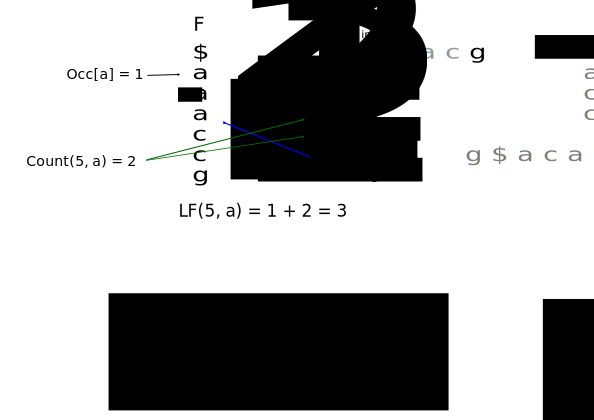
\includegraphics[scale = 0.5]{Figures/LF.png}
  \caption{LF-Mapping of $3^{rd}$ occurrence of $a$ from last column}
    \label{fig:LF}
\end{figure}
\end{minipage}
\begin{minipage}[t]{0.4\textwidth}
        This figure illustrates how the mapping is done : from the fact that character ranking are the same in both last and first column (and all the others for that matter), the \textsl{LF-Mapping} algorithm enables retrieval of the position in $F$ for any character in $L$. This method is used in the \textsl{Walk-Left} algorithm to reconstruct the original text, which is thereafter further detailed in figure \ref{fig:walkleft}.
\end{minipage}
\vspace*{5mm}

Finally, from a search point of view, the last property is the most interesting. Lexicographical order allows for spatial proximity of sought result, hence, an iterative search through a word to find in $T^{bwt}$ will see each iteration to indicate spatially close positions which yet facilitates this process.\\

Now that this concept is well defined, the next section will aim to illustrate how the FM-Index algorithm makes the best out of this transform in order to enable efficient data compression and sub-string queries.

\subsection{FM-Index}

An \textsl{FM-Index} is a lossless text compression based on the \textsl{BWT}\footcite{FM_INDEX}, it was created by \textsl{Paolo Ferragina} and \textsl{Giovanni Manzini} whom refer to it as an \textit{"opportunistic data structure"}. The design of this index is based upon the combination of the BWT and the suffix array data structure, displayed in red in figure \ref{fig:bwt}.\footnote{https://pdfs.semanticscholar.org/d896/e62b6cbfd623d1d9041f90b7f9e41d1451a7.pdf}

\paragraph{Creating an FM-Index}

In order to create the \textsl{FM-Index} of an input full-text \textit{string} $T$, one must create its \textsl{BWT} transform $T^{bwt}$ as explained in the previous section. Referring again to figure \ref{fig:bwt}, the \textcolor{red}{red} sub-matrix from the one in the middle, i.e. the suffix array (SA) will also be used. Finally, the index itself, noted $F$ will be constructed from the SA and $T^{bwt}$. \\

For a given $T^{bwt}$ of $N$ symbols on an alphabet $\Sigma$ of $\sigma$ elements, we define the FM-Index $F$ as a two-dimensional matrix with $(N + 1)$ rows and $\sigma$ column. Hence, the entry at index $i$ (row) and for symbol $c$ (column), $F[i][c]$ contains the number of occurrences of $c$ before the index $i$ in $T^{BWT}$. From this definition, we can construct the whole index for $T^{bwt}$, initializing $F[0]$ at $0$ and $\forall$ $i$ from $0$ to $N$, copy $F[i]$ into $F[i+1]$, incrementing $F[i+1][c]$ only if $T^{BWT}[i]$ = $c$. The last entry $F[N + 1]$ represents the total number of occurrences of all symbols in $T^{bwt}$. This whole structure of the FM-Index is given an example in the figure \ref{fig:fmindex} below. \\

\begin{minipage}{0.5\textwidth}
\begin{figure}[H]
    \hspace{-15mm}\includegraphics[scale = 0.35]{Figures/FMIndex.png}
    \caption{Illustration of the FM-Index construction from "$acaacg$}
    \label{fig:fmindex}
\end{figure}
\end{minipage}
\hspace{15mm}
\begin{minipage}{0.3\textwidth}
After applying the BWT to the input text, the suffix array is extracted and from it, the $Occ$ array. From the transform itself, the FM-Index $F$ is filled. \\
Note that in this case, $F$ replaces the function $Count$ described in the previous section by statically storing all those values a priori.
\end{minipage}


\paragraph{Walk-Left and String Matching Algorithms} In the scope of the FM-Index, it is at some point required to revert the BWT in order to determine the position of the queried string in the original text. To that end, the \textsl{LF-Mapping} algorithm introduced in the previous section shows is used in the definition of another algorithm, \textsl{Walk-Left}. This procedure, presented below, can be used to fully revert the transform, given $Occ$, the transform $T^{bwt}$ and the FM-Index $F$, as described in the algorithm below.

\begin{minipage}[t]{0.55\textwidth}
\begin{algorithm}[H]
	\SetAlgoLined
	\KwIn{BWT $T^{bwt}$, FM-Index $F$, First occurrences $Occ$}
	\KwOut{The original input string $T$}
	i = 0\;
	t = ""\;
	\While{$T^{bwt}[i] \neq $ "\$"}{
		t = $T^{BWT}[i] $ + t\;
		i = $LF(i, T^{BWT}[i])$\;
	}
\caption{Walk-Left - Inverting the BWT}
\end{algorithm}
\end{minipage}
\hspace{3mm}
\begin{minipage}[t]{0.3\textwidth}
This very simple algorithm starts from the $1^{st}$ character of $T^{bwt}$ and, until the $eos$ character \$ is reached, concatenates the current character $c$ to the result string and updates the index using LF-Mapping.

\end{minipage}
\vspace*{5mm}

\begin{figure}[H]
\centering
\includegraphics[scale = 0.4]{Figures/WL_algo.png}
\caption{Illustration of the Walk-Left Algorithm inverting the $T^{bwt}$ to retrieve original text $T$}
\label{fig:walkleft}
\end{figure}

Using the same function, we now define an algorithm that, given a BWT $T^{bwt}$ and a query string $q$, will return the index range in the implicit suffix array containing $q$ : \\

\begin{minipage}[t]{0.55\textwidth}
\begin{algorithm}[H]
\SetAlgoLined
\KwIn{BWT $T^{bwt}$, FM-Index $F$, First occurrences $Occ$, query string $q$}
\KwOut{Index Range $top$, $bot$ for $q$ in the suffix array corresponding to $T^{bwt}$ }
	$top$ = 0\;
	$bot$ = $len(T^{BWT})$\;
	\For{$qc$ in $reverse(q)$}{
		$top$ = $LF(top, qc)$\;
		$bot$ = $LF(bot, qc)$\;
}
\caption{Exact String Matching in Suffix Array}
\end{algorithm}
\end{minipage}
\hspace{3mm}
\begin{minipage}[t]{0.3\textwidth}
Blablablabla blabla bla bla bla bla bla
\end{minipage}

\begin{figure}[H]
\centering
\includegraphics[scale = 0.35]{Figures/matching_algo.png}
\caption{Illustration of the matching process of the string  $q$ = $"aac"$ in the suffix array derived from $T^{bwt}$ }
\end{figure}


If the return range $[top, bot]$ is empty, then the queried string $q$ does not appear in the reference text.


\paragraph{Putting it all Together}

Now that all the data structures and computational tools have been introduced, we can define the process of exact string matching using the FM-Index, in an input reference string $T$ and a string query $q$ :
\begin{enumerate}
\item Compute the Burrows-Wheeler Transform $T^{bwt}$ of $T$, use it to find $Occ$ and to get the FM-Index $F$.
\item Use Algorithm 2 to determine the index of the rotation in the implicit suffix array containing $q$
\item If such an index exists (i.e. $q$ occurs at least once in $T$), use the Walk-Left Algorithm to walk back to the beginning of the text from this index
\item The number of steps corresponds to the offset of $q$ in $T$
\end{enumerate}

\paragraph{Performance Analysis}

As mentioned earlier in this document, the size of a genomic dataset is usually in the billion of entry range. Hence, we consider the following items in the previously defined process to be way too costly time or space-wise : 
\begin{itemize}
	\item Step 4 of the procedure requires a number of step linear to the length of $T$. Doing this may require billions of iterations over the lines $4$ and $5$ of Algorithm 1, meaning billions of memory access, which is way too much time consuming.
	\item Storing the whole FM-Index requires storing $(N + 1)*\sigma$ values, with $N$ the length of $T$ and $\sigma$ the size of its alphabet $\Sigma$. This would require in our case at least 6 times the size of $T$ in memory space, which is way too big.
	\end{itemize}
	In order to reduce both those costs, the following solution is introduced :
	\begin{itemize}
		\item Keep samples of the suffix array index (e.g. every 32$^{th}$ row), when "walking" back along $T^{BWT}$ check if an entry exists for the current position, if yes, then add this value to the number of step already done to obtain the position of $q$ in $T$. This allows to Walk-Left algorithm to operate in a constant time, while limiting the space needed to store those values.
		\item Keep only some samples of the FM-Index (e.g. one every 128 entries), referred as " checkpoints ". The LF function would now take the index of the current symbol in $T^{bwt}$ and find the closest surrounding checkpoint, then "walk" along $T^{bwt}$, counting the occurrences of the same symbol along the way and adding/subtracting (respectively if the closest checkpoint is above or below the current index) this count to the rank value stored in the checkpoint. This reduces greatly the space needed to store the index, while keeping a constant computation time for the LF function.
		\end{itemize}
		
		\begin{figure}[h]
			\centering
			\begin{subfigure}{.5\textwidth}
				\centering
				\includegraphics[width=.5\linewidth]{Figures/sa.png}
				\caption{SA sample example}
				\label{fig:sub1}
				\end{subfigure}%
				\begin{subfigure}{.5\textwidth}
					\centering
					\includegraphics[width=.8\linewidth]{Figures/CHECKPOINT.png}
					\caption{Checkpoint example}
					\label{fig:sub2}
					\end{subfigure}
					\caption{Illustration of the two proposed improvement}
					\label{fig:test}
					\end{figure}
					
					Conclure
					
									

\section{Python Naive Implementation}

In order to get a better grasp of the concepts involved in the FM-Index implementation, a first one has been done in \textsl{Python}. The main advantage of this language is the syntax simplicity, allowing to focus on the algorithm and data-flow aspects of the string matching process while neglecting the data structures and global performances. \\

Good results have been reached using an adapted version of (CITER REPO), and this project has been used as a good basis for the less simple but way more precise \textsl{C++} implementation described in the next section. Below is a schema describing the software structure and execution flow.

[Poser un genre d'UML]

Using a terminal interface, the program is used as follow : 

[Mettre un screenshot]

\section{C++ Implementation}

All the software components of this project interacting with the board will be written in \textsl{C++}. This choice is based on legacy reasons (\textsl{REDS} environment) and conceptual reasons. The latter comes from the need to define a precise encoding of the \textsl{nucleotide reads} to be used on the FPGA system along with well defined and space-optimized data structures to store the \textsl{BWT} in the memory, the suffix array samples and the FM-Index checkpoints.

\subsection{Reads encoding and Data Structures}

\paragraph{Reads encoding}

Considering there are 4 different nucleotides within any DNA sequence, adding the uncalled base N type read and the "\$" equivalent character, we need to encode 6 symbols and thus need at least 3 bits. Therefore, it has been chose to use the following encoding : \\

\begin{minipage}[c]{0.35\textwidth}
\vspace*{6mm}
	\begin{tabular}{|c|l|}
	\hline
		Name & Encoding \\
		\hline 
		"\$" & 000 \\
		A & 010 \\
		C & 100 \\
		G & 101 \\
		T & 110 \\
		N & 111 \\
    \hline
	\end{tabular}
\end{minipage}
\begin{minipage}[t]{0.85\textwidth}
\vspace*{-30mm}
    \begin{minted}{c}
/* Type on 8 bits (only last 3 used) */
typedef unsigned char nucl_read; 
/* $ character */
static const nucl_read eos    = 0x00;	
static const nucl_read a_read = 0x02;
static const nucl_read c_read = 0x04;
static const nucl_read g_read = 0x05;
static const nucl_read t_read = 0x06;
static const nucl_read n_read = 0x07;
    \end{minted}
\begin{lstlisting}


\end{lstlisting}
\end{minipage}
\vspace*{3mm}

Dire un mot sur que quand meme voila c'est cool.
	

\paragraph{Data Structures}

Specific data structure will be needed in this program, not only to create the index and implement the whole algorithm, but also to be able to create files of a specific format containting the transform, the suffix array, etc. Those will then be used later with the hardware implementation of the index.

\begin{minipage}[t]{0.4\textwidth}
	\textbf{Checkpoint Entry -} \\
	\vspace{-5mm}
	\begin{minted}{c}   
typedef struct checkpoint_entry
{
    uint32_t eos_count = 0;
    uint32_t a_count   = 0;
    uint32_t c_count   = 0;
    uint32_t g_count   = 0;
    uint32_t t_count   = 0;
    uint32_t n_count   = 0;
	
} checkpoint_entry;
	\end{minted}
\end{minipage}
\hspace*{15mm}
\begin{minipage}[t]{0.5\textwidth}
		\textbf{BWT Class Attributes - }
\begin{minted}{c}
/* Last column = BWT(T) */
nucl_read * L;
/* First column of ordered SA */
nucl_read * F;	
/* First occurence array */
checkpoint_entry * occ;	
/* FM-Index samples */
checkpoint_entry * checkpoints; 
/* Sampled suffix array index's */
uint64_t * suffix_idx;	

	\end{minted}
	\textcolor{white}{.}\\

	
	
\end{minipage}
\vspace*{4mm}
Below is a schema describing the program structure and execution flow along with the files it produces from the FM-Index structures :

[Justifier les types, faire un UML ou quelque chose comme ca pour illustrer le fonctionnement]

Using a terminal interface, this program is used as follow :

[Poser un screenshot d'execution]


\section{Tests \& Validation}

[Benchmark pour C++ ??] 
% Chapter Template

\chapter{Hardware Sequential Implementation of the FM-Index} % Main chapter title

\label{Chapter3} % Change X to a consecutive number; for referencing this chapter elsewhere, use \ref{ChapterX}			
The main scope of this thesis is to implement the aforementioned algorithm on a specific \textsl{FPGA} board, with all the reference data stored in a memory accessible via bus interface. This chapter will aim to describe a first implementation of this algorithm that could be duplicated on one board and used in parallel.

\section{Conception}

%A first, sequential, model is presented in the Figures \ref{fig:seqschema} and \ref{fig:fsm}.\\
\begin{figure}[H]
    \centering
    \hspace*{-25mm}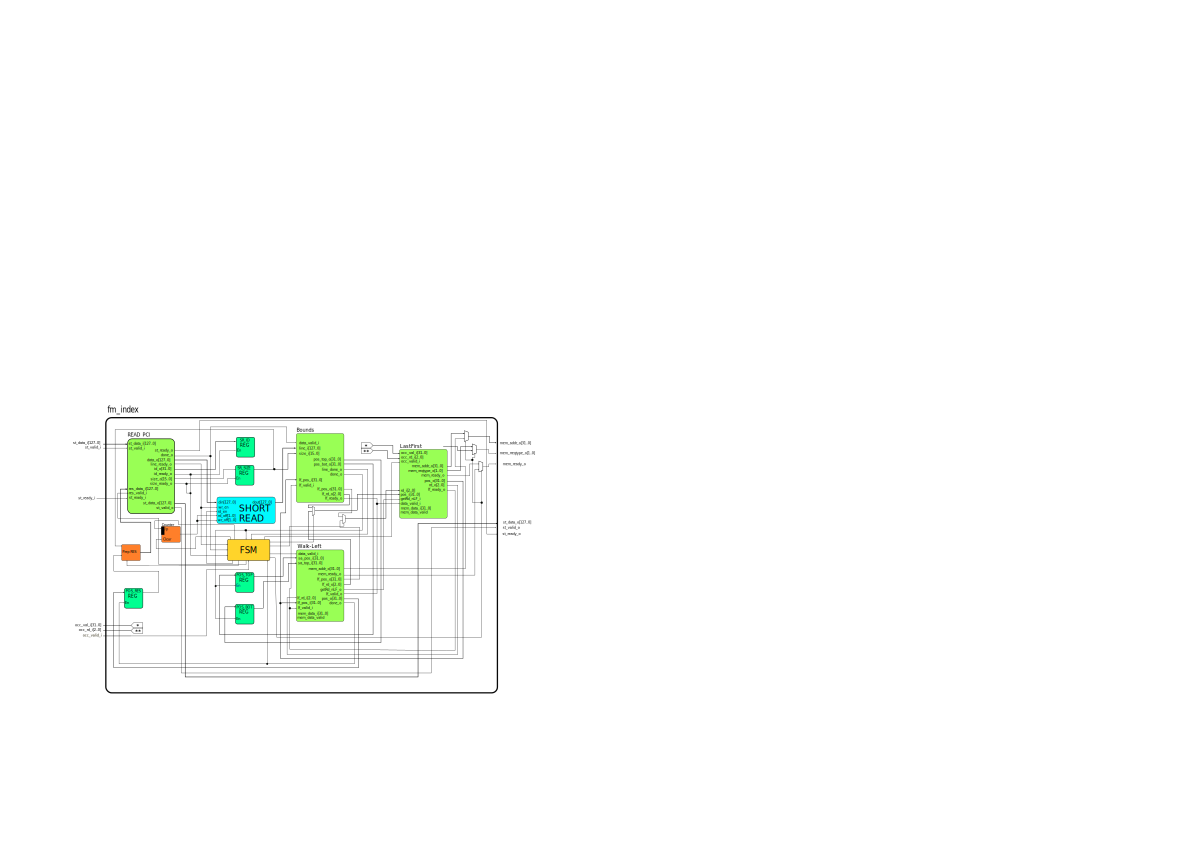
\includegraphics[scale = 0.45]{Figures/fmindex_top.png}
    \caption{Schema bloc of the FM-Index Top-Level}
    \label{fig:seqschema}
\end{figure}

Figures \ref{fig:seqschema} illustrate the hierarchy of the different blocks and element composing the \textsl{FM-Index}. \\

The details of the main FSM are described in Figure \ref{fig:fsm}, the different blocks are described in Section 3.1.2. Note that there are two different data input : one that is used to receive actual sequences to map onto the reference, the other is used to configure the \textsl{Occ} array, used in the LastFirst Mapping.

\subsection{FM-Index Global FSM}

This section illustrates the internal functioning of the \textsl{FM-Index} bloc, which is a hierarchical FSM, divided in 4 main steps as described below and illustrated in Figure \ref{fig:fsm}.
\begin{description}
\item [Read Sequence -] This loop is used to consume data from the \textsl{PCI Express Interface} in order to load a short read to align in the reference text along with an ID value associated to it.
\item [Bounds] - This loop scans the input sequence $q$ and, at each iteration, queries the \textsl{HMC} memory to update $top$ and $bot$. Note that is corresponds to Algorithm \ref{alg:match}.
\item [Walk Left] - This loop corresponds to Algorithm \ref{alg:WL}. It is only reached when the precedent loop ends up with a valid range for $q$ in the suffix array, i.e. $q$ exists in the reference text. Then again, at each iteration, the HMC is queried to update the index.
\item [Send Result] - This last part of the FSM sends back the results, whether $q$ was found or not, back to the result FIFO in the \textsl{PCI Express Interface}. This result contains the position (special value if not found), along with the ID corresponding to the query, stored in the \textsl{Read Sequence} step.
\end{description}
\begin{figure}[H]
 \includegraphics[scale = 0.4]{Figures/MSS.png}
    \caption{Global view of the FM-Index FSM}
    \label{fig:fsm}
\end{figure}

\subsection{ReadWrite\_Stream}

[SIMPLE SCHEMA BLOCK, FSM]

This block is responsible for reading the received data by the streaming bus. Those data start by the \textsl{short read} ID and size, followed by the actual sequence, already encoded and inverted. The first information are stored in registers and the short read itself is placed into a buffer : once a line is ready, the global FSM is notified, and the reading continue.

\subsection{Bounds}

[SIMPLE SCHEMA BLOCK, FSM] \\


 This block reads this sequence from the buffer on line at a time, once all elements from it have been used, it notifies the upper level it is ready for the next one and continues until it has read \textrm{size} elements. For each read symbol iteration, the top and bottom position outputs are updated one after the other. After each update, both the number of read symbol and the new positions are evaluated and just like in Algorithm \ref{alg:match}, if at some point the interval $ [ top,bottom ] $ is empty, the loop is terminated the FSM goes back to waiting for a new sequence.

\subsection{Walk-Left}

[SIMPLE SCHEMA BLOCK, FSM] \\

Upon termination of the \textsl{Bounds} algorithm, this block is notified that a new data is available. At the present time, only the \textsl{top} position is used. Hence, only one match - given there are at least one - is returned for each provided short read. As presented in Algorithm \ref{alg:WL}, this block first checks if there is a Suffix-Array index sample available for the provided position. If that's the case, it queries this value to the memory and returns it directly. If not, it fetches the BWT symbol corresponding to the current position and update this position using said symbol and said position for a LF-Mapping, and increments the number of step done so far. Then again, the new position is evaluated for a Suffix-Array index sample and so on and so forth until either the current position has such a sample, or the termination symbol \"\#\" is reached.
In the first case, the returned position is the number of step added to the index sample, in the latter, the number of steps is returned. \\

In both cases, the returned position corresponds to the short read position in the original (untransformed) text \textsl{T}.

\subsection{Last-First}

[SIMPLE SCHEMA BLOCK, FSM] \\

This block, used by both the \textsl{Bounds} and \textsl{Walk\_Left} blocks is the central processing unit of the FM-Index. This bloc aims to implement the mapping between the \textsl{BWT} symbols and their respective index in the conceptual suffix array first column (Equation \ref{eq:LF}. For each symbol of \textsl{T's} alphabet, its \textsl{Occ} value can be provided via a dedicated interface and placed into local registers. In order to determine the \textsl{Count} value of the provided inputs, it first queries the closest checkpoint value corresponding to the given symbol. It then iteratively queries \textsl{BWT} symbol from this position until it reaches the given position, incrementing a local count value each time the obtained symbol corresponds to the input.

Upon termination, the sum of all three values is returned. \\

Considering this methods of implementing \textsl{LF} requires querying symbols from the BWT, this block also provides this function to the rest of the system (only used by \textsl{Walk\_Left}, hence the input signal \textrm{getChar\_nLF\_i} that indicates which operation is demanded. To this end, an output signal \textrm{sbl\_o} is used to return the obtained symbol upon request.

\section{VHDL Implementation}

Mettre ici la figure d'avant, changer la figure d'avant pour enlever tous les trucs RTL : BRAM, REG, MUX et mettre juste des décideurs à la place.

Mettre RTL ?

\subsection{FMIndex}

\subsection{Read PCI}

\subsection{Last-First}

\subsection{Bounds}

\subsection{Walk-Left}



\section{Test \& Validation}

In order to validate the behavior of the whole system while keeping good handle of its complexity, a testbench suite has been developped for each bloc composing the system, with a final one for the whole \textsl{FM-Index} bloc. \\

\subsection{References}
To simulate the memory, a reference dataset has been created using the previously introduced software. Using a reference text of length 1000, all the elements have been computed and place in reference files :

\begin{description}
\item [bwt\_pkg -] This file contains an array of all the BWT symbols in correct orders
\item [ssa\_pkg -] This file contains an array of all the sampled Suffix-Array indices
\item [chkX\_pkg -] Those files, one for each symbol A, C, G, T, and N contains an array of all the sampled checkpoints for each of those.
\item [lfX\_pkg -] Like the previous files, each one of those contains a lookup-table of Eq. \ref{eq:LF} for each possible entry.
\end{description}

\subsection{Global Structure}

\begin{figure}[H]
 \includegraphics[scale = 0.4]{Figures/TB_struct.png}
    \caption{Global Structure of each Testbench}
    \label{fig:Tb_struct}
\end{figure}

Each testbench is defined according to the same structure, as depicted in Figure \ref{fig:Tb_struct}. For each DUT, a record is defined for each input sender and output receiver. For each input record, a process is defined to generate stimuli and for each output record, an equality operator is defined, allowing the \textrm{Verification} process to check the correctness of those output signals. \\
All DUT receive input from another internal block, referred as FM, which expects a final result. In order to get those results, most blocks need to interact with an external resource (such as a memory, a bus, etc.). Thus, those being independent in the computing process, it has been decided to completely separate those signals both in stimulation and verification. \\

Finally, every testbench includes two processes to generate a clock signal and an initial reset signal. The first is stop upon the termination of the FM-stimuli. \\

The following paragraphs further detail those different input and output for each block and summarize the operations performed.


\subsection{Read PCI}
\vspace*{3mm}
\begin{center}
    \begin{tabular}{|c|c|}
\hline
  Input Src   &  Description \\
  \hline
   Stream  & Incoming data from the computer master (short reads) \\
   FM-Index & Result data to send back and data request \\
   \hline
\end{tabular}
\end{center}
\vspace*{5mm}

Upon availability of incoming data from the stream, the block should consume it as soon as the FM-Index is ready to process a new sequence. The other way, upon availability of a result from the FM-Index, it should send it out on the stream as soon a it becomes available.
\begin{center}
\begin{tabular}{|c|c|}
\hline
  Output Dest   &  Description \\
  \hline
   Stream  & Result Data (position, id) \\
   FM-Index & Data to process (id, size, sequence) \\
   \hline
\end{tabular}
\end{center}
\vspace*{5mm}
Data from received from the stream should be parsed correctly before being sent out to the FM-Index, meaning extracting the sequence's size and ID from the first packet and then fill the buffer line by line according to the previously received size. The other way around, it should push on the bus the final results provided by the FM-Index. \\


Following those properties, two cases are implemented in order to fully verify them :
\begin{itemize}
    \item [-] Simulate an incoming sequence from the stream and verify the FM-Index outputs
    \item [-] Simulate incoming results from the FM-Index and verify the stream outputs.
\end{itemize}


\subsection{Bounds}
\vspace*{3mm}
\begin{center}
    \begin{tabular}{|c|c|}
\hline
  Input Src   &  Description \\
  \hline
   FM-Index  & Validity flag, sequence row and size \\
   Last-First & Position result from made requests \\
   \hline
\end{tabular}
\end{center}
\vspace*{5mm}

When a new sequence becomes available, the DUT should immediately start to scann it, starting from the initial positions and, for each symbol, update those position using the Last-First Mapping algorithm (Eq. \ref{eq:LF}). Upon the reception of such a result, it should either go to the next symbol, request the next line if the current has been scanned, or terminate if all the sequence has been read, returning the final \textsl{top} and \textsl{bottom} positions. Note that the termination of the algorithm might be caused by obtaining an empty range, in which case the DUT should not keep scanning. \\
\begin{center}
\begin{tabular}{|c|c|}
\hline
  Output Dest   &  Description \\
  \hline
   FM-Index  & Validity flag, sequence row and size \\
   Last-First & Position result from made requests \\
   \hline
\end{tabular}
\end{center}
\vspace*{5mm}
For each symbol in the sequence, the correct queries should be made to Last-First, meaning the correct position and symbol. Finally, upon termination of the algorithm, the correct position should be returned.

Following those properties, two cases are implemented in order to fully verify them, using the LF references to generate Last-First stimuli :
\begin{itemize}
    \item [-] Simulate an incoming sequence present in the text and generate LF results upon request. Upon termination, verify the position outputs.
    \item [-]  Simulate an incoming sequence not present in the text and generate LF results upon request. Make sure of the early termination (less loop iteration than there are symbol in the sequence).
\end{itemize}

\subsection{Last-First}

\vspace*{3mm}
\begin{center}
    \begin{tabular}{|c|c|}
\hline
  Input Src   &  Description \\
  \hline
   FM-Index  & Position, symbol and operation type \\
   Memory & Position or BWT line \\
   \hline
\end{tabular}
\end{center}
\vspace*{5mm}

Upon a new request, the DUT should prepare the correct request to the memory. Upon reception of requested data from memory, it should use it to correctly continue its execution.

\begin{center}
\begin{tabular}{|c|c|}
\hline
  Output Dest   &  Description \\
  \hline
   FM-Index  & Position or BWT symbol \\
   Last-First & Position or symbol \\
   Memory & Position and request type \\
   \hline
\end{tabular}
\end{center}

Depending on the desired data, either a checkpoint position or a sample of the BWT, the correct outputs should be given to the memory interface. Upon termination of the algorithm, the correct value should be given to the FM-Index.

Following those properties, two cases are implemented in order to fully verify them, using the checkpoints and BWT references to generate memory stimuli :
\begin{itemize}
    \item [-] Simulate a position request and verify the sequence of request made to the memory in addition to the final results. 
    \item [-] Do the same simulatin a symbol request.
\end{itemize}
\subsection{Walk-Left}

\vspace*{3mm}
\begin{center}
    \begin{tabular}{|c|c|}
\hline
  Input Src   &  Description \\
  \hline
   FM-Index  & Position, symbol and operation type \\
   Last-First & Position and symbol \\
   Memory & Suffix-Array sample \\
   \hline
\end{tabular}
\end{center}
\vspace*{5mm}

Upon the availability of new data, the DUT should start immediatly to execute its algorithm. It should updates internal registers upon reception of Last-First (and potentially terminate) and terminate upon reception of memory data (retrieving a Suffix-Array sample leading to the final result).

\begin{center}
\begin{tabular}{|c|c|}
\hline
  Output Dest   &  Description \\
  \hline
    FM-Index  & Position of the short read in the text \\
   Last-First & Position, symbol and request type
   Memory & Position \\
   \hline
\end{tabular}
\end{center}

The DUT algorithm should be able to query symbols and positions from Last-First and a Suffix-Array from the memory. Upon termination, it should provide the correct value to the FM-Index interface.

Following those properties, several cases involving multiple positions are implemented, using the Suffiy-Array, the LFs and BWT references to generate memory stimuli. A loop is then done on a pre-defined array of test values.

\subsection{FMIndex}

\vspace*{3mm}
\begin{center}
    \begin{tabular}{|c|c|c|}
\hline
  Interfaces & Direction  &  Description \\
  \hline
   Stream & In  & Short reads sequence with ID and size \\
   Stream & Out & Position in text T \\
   \hline
\end{tabular}
\end{center}
\vspace*{5mm}

Upon the availability of new data on the input stream, the DUT and its component should start to process those data. A result must be reached and sent on the ouput stream.

Using the checkpoints, Suffix-Array and BWT references to generate memory stimuli, two case are implemented, one involving a input present in the text, the position of which is then verified. And another one involving an input not present in the text.

\section{Results}

As a result of those tests and simulation, several timing issues have been detected. Indeed, the use of register to store the data and signals as flags to notify other blocks of data availability led to several synchronization problems. 

\begin{figure}[H]
    \centering
    \hspace*{-30mm}\includegraphics[scale = 0.4]{Figures/lf_timing_issue.png}
    \caption{Example of Signal and Data Synchronization Issue}
    \label{fig:lf_timing}
\end{figure}

Furthermore, 
% Chapter Template

\chapter{On-Board Integration} % Main chapter title

\label{Chapter4} % Change X to a consecutive number; for referencing this chapter elsewhere, use \ref{ChapterX}

%----------------------------------------------------------------------------------------
%	SECTION 1
%----------------------------------------------------------------------------------------

\section{Tools Introduction}

\subsection{Hybrid Memory Cube and Micron AC-510}


\textsl{Hybrid Memory Cube} (HMC) is a high-performance \textsl{RAM} interface for stacked \textsl{DRAM} memory. Combining \textsc{through-silicon vias} and \textsl{microbumps}\footnote{ (WIKIPEDIA) } to connect multiple layers of memory cells on top of each others, it offers very high throughput parallel serial bus' for random I/O's. In the scope of this project, it is an ideal candidate as to where to store all the references for the  FM-Index string matching algorithm as a parallel solution would indeed query for information potentially dispatched all over the memory.


\subsection{Board and Project Architecture}

The board introduced in the previous section is presented in Figure \ref{fig:board_schema}. It actually consists of 6 \textsl{AC-510} boards plugged onto a \textsl{EX-700} carrier board. This enables simultaneous use of several \textsl{AC-510} with one host connected by one bus. \\

In the project architecture for each \textsl{AC-510} board, several pre-defined \textsl{IPs}, provided by the board manufacturer, are used. A diagram representing the whole project hierarchy and coarse interconnections is presented in Figure \ref{fig:block_diag}. The different \textsl{IPs} and blocks have the following utility\footnote{Picodoc} :


\begin{description}
\item [HMC Controller] - This block offers an interface with the \textsl{HMC} internally for the \textsl{FPGA}, but also directly from the host (via PCIe), through the \textsl{FPGA}. Everything that comes and goes to the \textsl{HMC} passes through this block
\item [HMC Stream Controller ] - This blocks mainly has the same purpose that the previous one, except that it enables the communication between the \textsl{Pico-FrameWork} buses and the \textsl{HMC}.
\item [Pico Framework] - This \textsl{IP} provides a memory-mapped bus, the  \textsl{PicoBus}. It is used to initialize the \textsl{AC-510} device as well as configuring and using it via control/status registers and an PCIe bus.
\item [Pico Stream Controller] - This block, as well as the \textsl{HMC Stream Controler}, is used as an interface between a \textrm{256-bit} wide stream bus and an adapted \textrm{128bits} wide bus, used by the internal modules (e.g. \textsl{reds\_top}. This conversion is also necessary for the \textsl{HMC Stream Controller} to communicate  \textsl{PicoBus} data to/from the \textsl{HMC}.
\item [UserWrapper] - This block, as its name states, is used as a wrapper for any user application in the project. It enables a hierarchical architecture, much simpler to read and use, providing only the "stream adapters" \textsl{HMC Stream Contoller} and \textit{Pico Stream Controller}.
\item [Reds\_top \& FM-Index\_top ] - Those blocks are mainly used to keep a good hierarchical design by encapsulating case specific blocs in the global reusable project.
\end{description}


\begin{figure}[H]
    \centering
    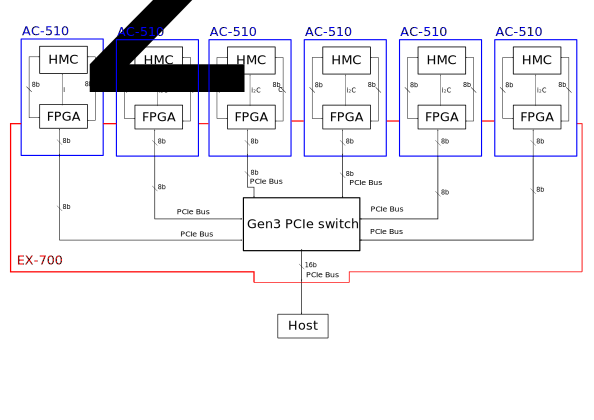
\includegraphics[scale = 0.4]{Figures/pico_board.png}
    \caption{Bloc Diagram of the Board}
    \label{fig:board_schema}
\end{figure}

\begin{minipage}[t]{0.6\textwidth}
\begin{figure}[H]
  \hspace{-15mm}  \includegraphics[scale = 0.6]{Figures/block_diagram.png}
    \caption{Bloc Diagram of the whole project}
    \label{fig:block_diag}
\end{figure}
\end{minipage}
\begin{minipage}[t]{0.35\textwidth}
Below are defined the differents references places on the Figures \ref{fig:block_diag} :
\begin{description}
\item [1] PCIe bus interface around the HMC controller, different from the \textrm{128-bit} wide bus used internally
\item [2] 8 parallel PCIe serial bus' for the \textsl{Pico Framework}, directly accessible from the host.
\item [3] Internal \textrm{256-bit} wide bus used to communicate with the lower-level design and the HMC.
\item [4] Internal \textrm{128-bit} wide bus used to communicate with the lower-level entity designed in this project and the \textsl{PicoBus}
\item [5] Internal \textrm{128-bit} wide bus used to communicate between the lower-level design and upper-level entities (e.g. host)
\item [6] \textrm{32-bit} wide direct bus between the \textsl{HMC Controller} and the lower-level entity designed in this project.
\end{description}
\end{minipage}

\section{Integration into the PicoBaseProject}


\subsection{Additional Blocs}



\begin{description}
\item [PCI Interface] - This bloc is the interface between the \textsl{PCI Express Bus} and the FM-Index bloc. It receives short reads and command from a master. In this interface, the FM-Index bloc is a slave, that wait for commands and data to start working. A FIFO is already implemented and this bloc consumes what is put into it. When a result is ready, it is placed in another FIFO that can be accessed by the computer master on the other end.
\item[Pico Bus Interface] - In order to enable addressed registers to configure the \textit{Occ} and \textit{LEN\_BWT} parameters, it seemed necessary to implement an interface to the PicoBus. The particularity of this bus is that it does not share the same clock that the rest of the system. It has indeed its own clock, expected to be much slower that the main one. This requires some level of synchronization in order to ensure the absence of metastable state of the written values. Thus, this bloc is in charge of listening to the address bus of the PicoBus interface in order to detect software originated writes. If one of those transaction is destined to one of the FM-Index internal parameters, it forwards the correct values to the central bloc.
\item [HMC Interface] - Similarly to the first bloc, this one is the interface between the board main memory and the FM-Index bloc. Only accessed through the \textsl{Memory Query} bloc, it is used to query data, may it be checkpoints entries, BWT entries of Sampled Suffix array elements. All transactions are 128-bit wide and the interpretation of the received data in the \textsl{Memory Query} bloc.
\item [Memory Query] - This bloc is used by the FM-Index to issue all the different queries it might need along the string matching process, which means it implements all 3 "functions" needed by the FM-Index : $Occ$, $Count$ (thus $LF$) and $Walk-Left$ (with the sampled suffix array). Those queries can be about "checkpoints", BWT symbol or sampled suffix array entries and the type of said requests is specified by the \textrm{req\_type} signal. This bloc is then responsible for interpreting the received data and transmitting it in the appropriate form to the FM-Index bloc. Note that in the actual implementation, this bloc is part og the HMC Interface bloc.
\end{description}

\subsection{Reds\_Top}
\begin{figure}[H]
    \centering
    \includegraphics[scale = 0.55]{Figures/REDS_TOP_DIAG.png}
    \caption{reds\_top Bloc Diagram}
    \label{fig:reds_top_diag}
\end{figure}

\subsection{PCI Interface}

\begin{figure}[H]
    \centering
    \includegraphics[scale = 0.4]{Figures/PCI_INTFCE_DIAG.png}
    \caption{PCI Interface Bloc Diagram}
    \label{fig:pci_diag}
\end{figure}

\begin{minipage}[t]{0.45\textwidth}
\begin{figure}[H]
    \centering
    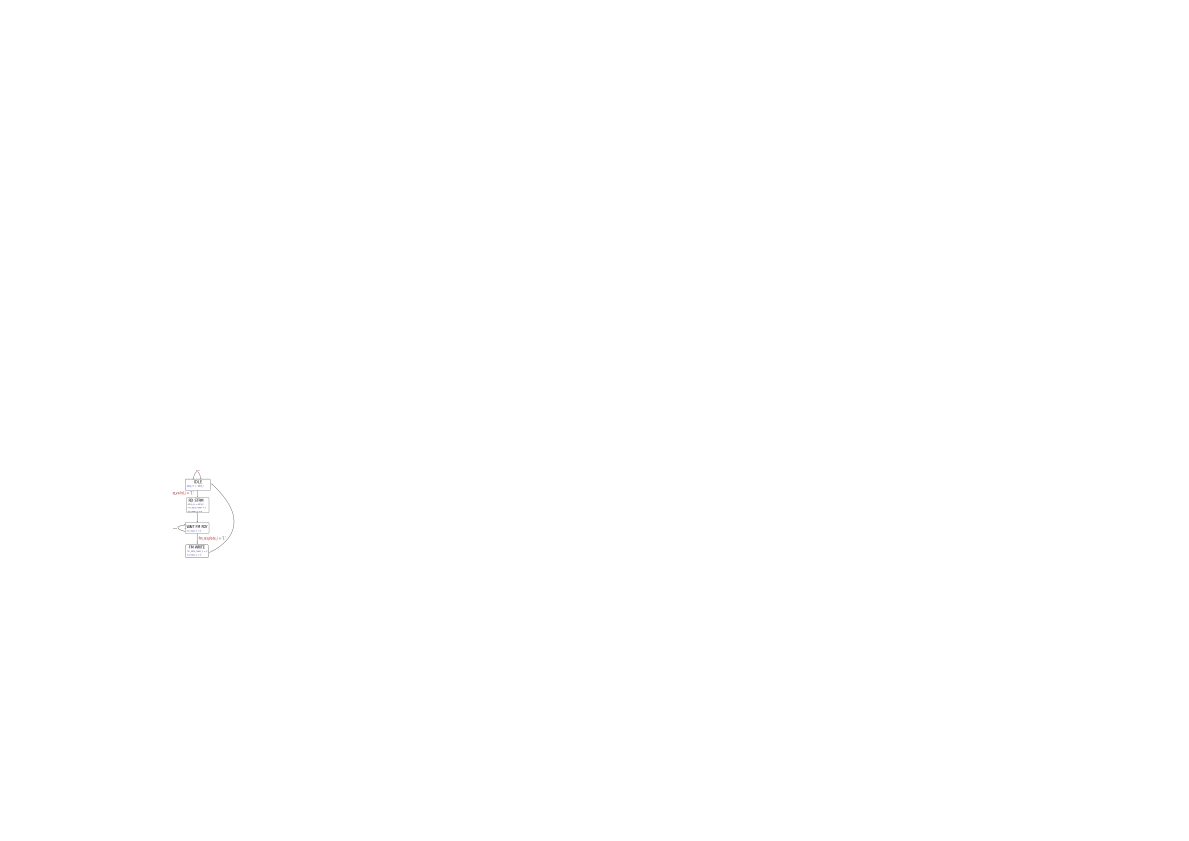
\includegraphics[scale = 0.4]{Figures/PCI_INTFCE_FSM.png}
    \caption{PCI Interface Bloc Diagram}
    \label{fig:pci_fsm}
\end{figure}
\end{minipage}
\hfill
\begin{minipage}[t]{0.3\textwidth}
This bloc keeps the received data into registers, await for the corresponding consumer to be ready. Two independent FSM are present, one for writing to the stream and of for reading from it. Both states machines are further detailed in Figure \ref{fig:pci_fsm}.
\end{minipage}


\subsection{PicoBus Interface}
\begin{figure}[H]
    \centering
    \hspace*{-20mm}\includegraphics[scale = 0.4]{Figures/REG_DIAG.png}
    \caption{PicoBus Interface Block Diagram}
    \label{fig:REG_DIAG}
\end{figure}

As mentioned earlier, a dedicated block is necessary to provide addressed register to the PicoBus. In Figure \ref{fig:REG_DIAG}, we can wee 3 layers of muxes and two layers of registers for each output signal. The first layer of muxes is used to enable updates only upon a write command from the bus. The second layer is used to update only the output corresponding to the provided address. The third layer is controled by the bus' clock, PicoClk in order for the update to by synchronized with the signal. This guarantees that, so far, all values are stable when forwarded. \\
Then, the first layer of registers is also clocked with the bus' clock, to avoid any meta-stability from between the precedent mux and this register. Finally, the last register layer is clocked by the system clock, so that the output are synchronized with the rest of the system. \\


\subsection{HMC Interface}

\begin{figure}[H]
    \centering
    \hspace*{-10mm}\includegraphics[scale = 0.35]{Figures/HMC_DIAG.png}
    \caption{HMC Interface Bloc Diagram}
    \label{fig:HMC_DIAG}
\end{figure}


\begin{minipage}[t]{0.5\textwidth}
\begin{figure}[H]
    \centering
    \hspace*{-10mm}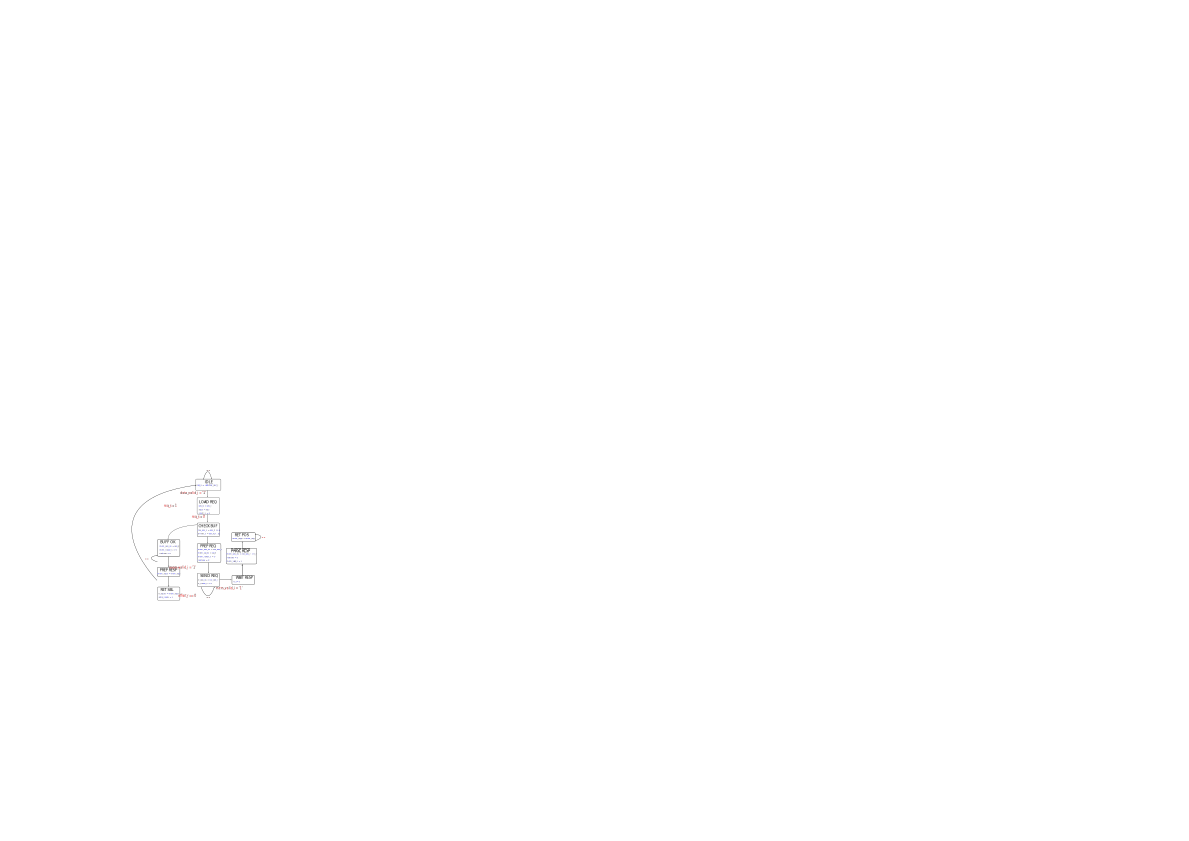
\includegraphics[scale = 0.35]{Figures/HMC_FSM.png}
    \caption{HMC Interface FSM}
    \label{fig:HMC_FSM}
\end{figure}
\end{minipage}
\hfill
\begin{minipage}[t]{0.4\textwidth}
The HMC interface waits for a request from a FM-Index. Upon such a requests, it loads the parameters in order to prepare the address to be sent to the HMC Controller. After sending the command, it waits for the response. Once the response is there, it stores the value in a local register before parsing it, depending on the FM-Index request parameters. Figure \ref{fig:HMC_FSM} further illustrates the process.
\end{minipage}

\subsection{Timing Requirements}

Inherited from the project are the timing requirements for the system, set at 250MHz, meaning that in order to produce a bitmap for the FPGA that would be guaranteed to behave as written, there should be no paths longer than 4 ns for a signal between two storing elements or port. \\
Considering the global structure of the implemented system, most paths respect this constraint as most exchanged data are stored into local registers and most operations are simple.\\

Nonetheless, the HMC Interface bloc had a path that did not last under that 4 ns, this being due to a rather unpleasant but necessary operation done one the position provided by the FM-Index. In the case of a query for a symbol of the BWT, the actual address is calculated by dividing this position by the number of symbol contained in each row, meaning here the inconvenient number 42. This kind of division is synthesized into a series of numerous simpler operations (see Fig. \ref{fig:timing}) with by default no storage element in between, thus creating a long path upon which we have little to no control. \\

\begin{figure}[H]
    \centering
    \hspace*{-3mm}\includegraphics[scale = 0.4]{Figures/TIMING_RTL.png}
    \caption{RTL View of the hardware path generated}
    \label{fig:timing}
\end{figure}
TODO
After some digging [REFORMULER] it was enough to enable more control to the synthesizer on the timings and optimization of those kind of delays to reduce this time to just under 4 ns. 

Another solution would have been to simplify the problematic operation by encoding the BWT on 4 bits. This would have allowed 32 elements per memory row, and thus reducing the division to a simple 5-bit shift to the right in order to determine an element's row and its position in it. However, this would have increase the space needed to store 

\section{C++ Interface Implementation}

In order to be able to communicate with the board from a computer, it requires a interface enabling :
\begin{itemize}
    \item [-] writing directly into the main memory in order to store the references
    \item [-]writing parameters to addressed registers
    \item [-] sending the short reads via a stream
    \item [-] reading the results via a stream
\end{itemize}

Furthermore, it becomes necessary to generate references that would correspond to their usage in the hardware system, hence providing methods that would not only encode those references (BWT, sampled suffix-array and checkpoints) but also write those correctly into the HMC. Figure \ref{fig:memory} show the memory organization. Each row is 128-bit, little endian. \\

The first point will be further discussed in the section PicoFramework, as it highly relies on the framework provided by the board manufacturer.

\begin{minipage}[t]{0.4\textwidth}
\begin{figure}[H]
    \centering
    \hspace*{-10mm}\includegraphics[scale = 0.4]{Figures/MEM_RPZ.png}
    \caption{Memory Organization}
    \label{fig:memory}
\end{figure}
\end{minipage}
\hfill
\begin{minipage}[t]{0.5\textwidth}

The biggest reference to store is the BWT with 3-bit values for each symbol, half of the memory is dedicated to it. \\
Then, the Sampled Suffix-Array with 32-bit values every 32 symbols (average 1 bit per symbol). \\
Finally the checkpoints, separated by symbol in order to simplify the address and the offset calculation, although it requires passing the requested symbol to the HMC Interface. For 5 symbols, it requires $5 * 32 / 128$ bits, so an average of 1.25 bit per symbol.\\
Hence, a total of 5.25 bits per symbol is necessary to store all the references, with a 4GiB memory, we can then process references up to $\approx 8.2*10^{8}$ symbols.
\end{minipage}

\vspace*{8mm}

\paragraph{BWT encoding}

In order to correctly encode the BWT, the number of element per row has to be taken into account. Considering there is no 128-bit integer type available to store data row per row, each one of those is split into two 64-bit unsigned integers. Considering the symbols are encoded on 3 bits, there is no way to fill each word with a round number of symbols. Hence, in order to keep the data coherent, for each row, the procedure is describer in Algorithm \ref{alg:bwt}.\\


\vspace*{5mm}


\begin{minipage}[t]{0.55\textwidth}
\begin{algorithm}[H]
	\SetAlgoLined
	\KwIn{BWT $T^{bwt}$ encoded as in section 2.3.1}
	\KwOut{vector of uint64\_t pairs}
	res = <>; \textit{\# Empty vector of uint64\_t pairs} \\
	temp = <>; \textit{\# Empty pair of uint64\_t} \\
	j = 0; \textit{\# Global Index}\\
	\For{each 42 symbols roW in $T^{bwt}$}{
		t = ""; \\
		\For{i = 0; i < 42; i++}{
		    t = to\_string(bwt[j]) + t;\\
		    j++;
		}
		temp[0] = str\_to\_integer(t[64..127], 2);
		temp[1] = str\_to\_integer(t[0..63], 2);
        res.append(temp);
	}
\caption{Encoding the BWT for Memory
}
\label{alg:bwt}
\end{algorithm}
\end{minipage}
 \hfill
\begin{minipage}[t]{0.3 \textwidth}
The string representation of each value is shown in the table below.
\vspace*{5mm}


\begin{tabular}{|c|c|}
\hline
Input    &  to\_string() result\\
\hline
 A    &  "010" \\
 C    &  "011" \\
 G    &  "100" \\
 N    &  "101" \\
 T    &  "110" \\
\hline
\end{tabular}
\vspace*{3mm}

The function \textit{str\_to\_integer} is given a string that it converts into an integer using the base provided as second argument to do the conversion. \\
\end{minipage}
\vspace*{5mm}


\textit{\underline{Note}} : If the number of symbols is not a multiple of 42, a last loop is done with the remainings values, padding the rest of the buffer row with '0's. \\



A string representation of each row must be done in order to correctly dispatch the bits between the two 64-bit words. Every string is constructed from the right to the left in order to place the first character where the least significant bits are (as it is interpreted by the conversion method - little endian). \\
Finally, the first element of each pair must represent the first 64 bits of the memory row, hence the indices [64..127] for the first 64-bit word, and [0..63] for the second that will be used for bits [63..0] and [127..64] respectively to write the memory row.

\paragraph{Sampled Suffix-Array and Checkpoints encoding}

All values from those references are stored in and used as 32-bit values. This round number allows 4 values per row and the order in which the written buffer is defined as follow :
\begin{enumerate}
    \item Fetch the next 4 values in an array \texttt{position[4]} of unsigned 32-bit integers with \texttt{position[0]} being the first fetched, etc.
    \item Convert each value into an hexadecimal representation
    \item Add this row to the final buffer
    \item Repeat from Step 1 until there is no value left
\end{enumerate}

\textit{\underline{Note}}: If the number of checkpoints or suffix-array sample is not a multiple of 4, this a last loop is done, padding the rest of the buffer row with '0's. \\

Both those encoding methods are passed a binary input file containing unsigned integer value for each position / symbol.

In the scope of this project, only a terminal interface will be implemented. It is used as follow :
\begin{enumerate}
    \item Launch the program providing either a bitmap or a project file corresponding to the system implemented for the FPGA
    \item Upon request, provide a FASTA file containing the reference genome
    \item Upon request, provide a FASTQ file containing the short reads to map onto the reference
    \item Upon notification, a text file should contain all the short reads reference followed by their position in the reference ('-1' if not found)
\end{enumerate}

The first step is further explained in the next section, as it fully takes advantage of the tools from the Pico Framework.


\subsection{Pico Framework}

This framework, provided by the board manufacturer, not only offers methods and tools to communicate with the board, but also a powerful way to simulate it and its execution. All the informations provided below are from the \textit{Pico User Guide}\cite{PICOO}.

\paragraph{Reaching the FPGA}
\begin{minted}{c}
PicoDrv *pico_ptr;
int FindPico(uint32_t model, PicoDrv **drvpp);
int RunBitFile(const char *bitFilePath, PicoDrv **drvpp);
\end{minted}

In order to be able to detect and link the FPGA, it is first necessary to declare a \texttt{PicoDrv} instance that will then provide all the methods in the next paragraphs. \\
The pointer is instantiated using the \texttt{FinPico} method, providing it also an index corresponding to the FPGA model (\texttt{0x510} in this project).\\
Then, the method \texttt{RunBitFile}, provided the aforementioned pointer and the path to a bitStream file, is used to program the FPGA with a compiled hardware system. \\
Note that this last method can also be provided a project descriptor (Vivado or Quartus) in order to launch a simulation. This aspect will be further discussed in Section 4.4.


\paragraph{Writing to the Memory} \\
\begin{minted}{c}
int WriteRam(uint64_t addr, const void * buf, int size, int memID);
\end{minted}
The address provided must be 16-Byte align, along with \texttt{buf} containing the data to write. Further more, \texttt{size} represents the number of bytes to write, it must also be a multiple of 16. Finally, \texttt{memID} indicates the ID of the memory to which we want to write, in this project, the required value is 0. \\

The first word of the buffer will be placed at the first byte of the memory row, hence the buffer is big-endian word-wise. For each word however, the value is read as a little endian.

\paragraph{Writing to and Ready from the Stream}
\begin{minted}{c}
int createStream(int streamID);
int ReadStream(int streamHandle, void * buf, size_t count);
int WriteStream(int streamHandle, const void * buf, size_t count);
\end{minted}
The first method is used to instanciate a handler for the stream that will then be needed for the two other methods. \\

The two following methods are used to respectively write to and read from the PCI stream between the computer and the FPGA. Considering the bus is a stream in this case, there are no addresses to provide but the \texttt{count} value is still required to be a multiple of the stream width in bytes, in this case, 16.

\section{Co-Simulation}

In order to facilitate the debug process, the Pico Framework offers a way to simulate the board instead of loading it to test the developped application. Doing so is rather simple : it is enough to provide the program a project file (e.g. \texttt{.fwproj} for Vivado, \texttt{.qpf} for Quartus).\\

This allowed us to thoroughly test the implemented system with a simulation very close to the reality. Despite being hard to read, the simulation provides all the desired signals inside the system, thus allowing for a deep inspection of its behavior.

\subsection{Constated Issues}

As a result to those simulations, several issues have been noted that did not occur in the previously mentioned testbenches :
\begin{itemize}
    \item [-] The endianness of the memory must be dealt with in order for the data to be coherent. Unexpectedly, it was a major issue during the test phase and on several occasions was the reason the system was failing.
    \item [-] The HMC memory bus' contain all '0' when not used. The requested data is only available for 1 clock period and thus, has to be latched immediately.
    \item [-] The PicoBus, from which the parameters registers are written, not only is used by the framework and thus, the address decoder must be restricted to a certain address range. But it also has a clock very much slower than the internal system clock. Hence, it is necessary deal with this by re-synchronizing the received data.
\end{itemize}

\section{On-Board Testing}

In order to test the system directly on the board, the same program can be used. Instead of providing it a project file, it is necessary to provide it a bitmap for the FPGA. If the FPGA is reachable, the test software will then proceed to program it and behave like in the simulation. \\

As expected, the result were the same than in the simulation.

\section{Validation}

In order to validate the system, the reference used in Chapter 3 has been used and some mock short reads extracted from it are used as input, this time, as is (meaning here as a text and not already processed data). \\

The results were quite satisfying, as all the bugs had been detected during the simulation process. \\

Despite being a little over the restriction (less than 0.1 ns) for a couple a paths, the system seems to behave correctly in normal conditions (low temperature and low demand).

% Chapter Template

\chapter{Project Results} % Main chapter title

\label{Chapter5} % Change X to a consecutive number; for referencing this chapter elsewhere, use \ref{ChapterX}

%----------------------------------------------------------------------------------------
%	SECTION 1
%----------------------------------------------------------------------------------------

Globally, the results obtained by the whole system (software and hardware) is satisfying. It is able to correctly index a reference and then search for a single exact match for each short read then provided and give a result back. \\

\section{Software}

\section{Hardware}

\section{Full System}


 
% Chapter Template

\chapter{Project Status and Possible Improvements} % Main chapter title

\label{Chapter6} % Change X to a consecutive number; for referencing this chapter elsewhere, use \ref{ChapterX}

%----------------------------------------------------------------------------------------
%	SECTION 1
%----------------------------------------------------------------------------------------





 
% Chapter Template

\chapter{Conclusion} % Main chapter title

\label{Conclusion} % Change X to a consecutive number; for referencing this chapter elsewhere, use \ref{ChapterX}

%----------------------------------------------------------------------------------------
%	SECTION 1
%----------------------------------------------------------------------------------------
\section{Project Status and Possible Improvements}
 


\section{Personal Comment}



\section{Acknowledgment}
 THANK YOU <3
%% Chapter Template

\addchaptertocentry{Bibliography}

\label{Biblio} % Change X to a consecutive number; for referencing this chapter elsewhere, use \ref{ChapterX}

%----------------------------------------------------------------------------------------
%	SECTION 1
%----------------------------------------------------------------------------------------
\begin{thebibliography}{9}

\bibitem{lamport94}
 Bashford, J. N., Norwood, J., \& Chapman, S. R. (1998). Why are patients prescribed proton pump inhibitors? Retrospective analysis of link between morbidity and prescribing in the General Practice Research Database. \textit{British Medical Journal, 317}(7156), 452-456. 
  
  \bibitem{lamport93}
 Bourne, C., Charpiat, B., Charhon, N., Bertin, C., Gouraud, A., Mouchoux, C., \& Janoly-Dumenil, A. (2013). Effets indésirables émergents des inhibiteurs de la pompe à protons. \textit{ Presse Médicale, 42}(2), e53-e62. 
  
  \bibitem{lamport92}
  Cunningham, R., Dale, B., Undy, B., \& Gaunt, N. (2003). Proton pump inhibitors as a risk factor for Clostridium difficile diarrhoea. \textit{Journal of Hospital Infection, 54}(3), 243-245. 
  
  \bibitem{lamport91}
  Dial, S., Alrasadi, K., Manoukian, C., Huang, A., \& Menzies, D. (2004). Risk of Clostridium difficile diarrhea among hospital inpatients prescribed proton pump inhibitors: cohort and case–control studies. \textit{Canadian Medical Association Journal, 171}(1), 33-38. 
  
  \bibitem{lamport90}
  Festinger, L. (1950). Informal social communication. \textit{Psychological review, 57}(5), 271-282. 
  
\bibitem{lamport89}
  Festinger, L. (1954). A theory of social comparison processes. \textit{Human relations, 7}(2), 117-140. 
  
  \bibitem{lamport88}
 Forgacs, I., \& Loganayagam, A. (2008). Overprescribing proton pump inhibitors. \textit{British Medical Journal, 28}(7634), 2-3. 
  
  \bibitem{lamport87}
  Leslie Lamport,
  \textit{\LaTeX: a document preparation system},
  Addison Wesley, Massachusetts,
  2nd edition,
  1994.
  
  \bibitem{lamport941}
 Freidson, E. (1984). \textit{La Profession Médicale}. Paris : Payot. 
  
  \bibitem{lamport942}
  Giger, J.-C. (2008). Examen critique du caractère prédictif, causal et falsifiable de deux théories de la relation attitude-comportement: la théorie de l’action raisonnée et la théorie du comportement planifié. \textit{L'année Psychologique, 108}(1), 107-131. 
  
  \bibitem{lamport924}
  Giuliano, C., Wilhelm, S. M., \& Kale-Pradhan, P. B. (2012). Are proton pump inhibitors associated with the development of community-acquired pneumonia? A meta-analysis.\textit{ Expert review of clinical pharmacology, 5}(3), 337-344. 
  
\bibitem{lamport934}
  Gulmez, S. E., Holm, A., Frederiksen, H., Jensen, T. G., \& Hallas, J. (2007). Use of proton pump inhibitors and the risk of community-acquired pneumonia: a population-based case-control study. \textit{Archives of Internal Medicine, 167}(9), 950-955. 
  
  \bibitem{lamport944}
  Haenisch, B., von Holt, K., Wiese, B., Prokein, J., Lange, C., Ernst, A., . . . Weyerer, S. (2015). Risk of dementia in elderly patients with the use of proton pump inhibitors.\textit{European archives of psychiatry and clinical neuroscience, 265}(5), 419-428.
  
  \bibitem{lamport954}
 Hallsworth, M., Chadborn, T., Sallis, A., Sanders, M., Berry, D., Greaves, F., \& Davies, S. C. (2016). Provision of social norm feedback to high prescribers of antibiotics in general practice: a pragmatic national randomised controlled trial. \textit{The Lancet, 387}(10029), 1743-1752. 
  
  \bibitem{lamport794}
  Heidelbaugh, J. J., Goldberg, K. L., \& Inadomi, J. M. (2009). Overutilization of proton pump inhibitors: a review of cost-effectiveness and risk in PPI. \textit{The American journal of gastroenterology, 104}, S27-S32. 
  
  \bibitem{lamport9334}
  Herghelegiu, A. M., Prada, G. I., \& Nacu, R. (2016). Prolonged use of proton pomp inhibitors and cognitive function in older adults. \textit{Farmacia Hospitalaria, 64}(2), 262-267. 
  
  \bibitem{lamport1294}
 Herranz, M. P. (2016). Is there an overprescription of proton pump inhibitors in oncohematologic patients undergoing ambulatory oncospecific treatment? \textit{Farmacia Hospitalaria, 40}(5), 436-446. 
 
\bibitem{lamport9554}
 Katz, J. (1984). Why doctors don't disclose uncertainty. \textit{Hastings Center Report, 14}(1), 35-44. 
  
  \bibitem{lampor33t94}
 Lam, J. R., Schneider, J. L., Zhao, W., \& Corley, D. A. (2013). Proton pump inhibitor and histamine 2 receptor antagonist use and vitamin B12 deficiency. \textit{Jama, 310}(22), 2435-2442. 
  
  \bibitem{lamport4594}
  Leyens, J.-P., \& Yzerbyt, V. (1997). \textit{Psychologie sociale}. Bruxelles : Editions Mardaga.
  
  \bibitem{lamport9er4}
 Maffei, M., Desmeules, J., Cereda, J., \& Hadengue, A. (2007). Effets indésirables des inhibiteurs de la pompe à protons (IPP). \textit{Revue médicale suisse, 3}(123), 1934-1938. 
  
  \bibitem{lampoet94}
 Martin, R. M., Dunn, N. R., Freemantle, S., \& Shakir, S. (2000). The rates of common adverse events reported during treatment with proton pump inhibitors used in general practice in England: cohort studies. \textit{British journal of clinical pharmacology, 50}(4), 366-372. 
  
  \bibitem{lamp324ort94}
  Nouguez, E. (2007). La définition des médicaments génériques entre enjeux thérapeutiques et économiques: L'exemple du marché français des inhibiteurs de la pompe à protons. \textit{Revue française des affaires sociales}, 3, 99-121. 
  
\bibitem{lawwmport94}
  Pollock, K., \& Grime, J. (2003). The cost and cost-effectiveness of PPIs: GP perspectives and responses to a prescribing dilemma and their implications for the development of patient-centred healthcare. \textit{The European journal of general practice, 9}(4), 126-133. 
  
  \bibitem{lampewort94}
 Reimer, C., Søndergaard, B., Hilsted, L., \& Bytzer, P. (2009). Proton-pump inhibitor therapy induces acid-related symptoms in healthy volunteers after withdrawal of therapy. \textit{Gastroenterology, 137}(1), 80-87. 
  
  \bibitem{laddmport94}
  Reinberg, O. (2015). Inhibiteurs de la pompe à protons (IPP): peut-être pas si inoffensifs que cela. \textit{Revue Medicale Suisse, 485}(11), 1665-1671. 
  
  \bibitem{laeemport94}
  Roulet, L., Vernaz, N., Giostra, E., Gasche, Y., \& Desmeules, J. (2012). Effets indésirables des inhibiteurs de la pompe à proton: faut-il craindre de les prescrire au long cours? \textit{La Revue de médecine interne, 33}(8), 439-445. 
  
  \bibitem{lampogtrt94}
  Sanduleanu, S., Stridsberg, M., Jonkers, D., Hameeteman, W., Biemond, I., Lundqvist, G., \& Stockbrügger, R. (1999). Serum gastrin and chromogranin A during medium-and long-term acid suppressive therapy: a case-control study. \textit{Alimentary Pharmacology and Therapeutics, 13}(2), 145-154. 
  
  \bibitem{ldemport94}
  Steuerwald, M., \& Meier, R. (2003). Troubles peptiques (2e partie): Ulcères peptiques. \textit{Forum Medical Suisse, 3}(42), 1008-1012. 
  
  \bibitem{lampfrort94}
  Thomson, A. B., Sauve, M. D., Kassam, N., \& Kamitakahara, H. (2010). Safety of the long-term use of proton pump inhibitors. \textit{World Journal of Gastroenterology, 16}(19), 2323-2330
  
  \bibitem{lampotgrt94}
  Turner, J. C. (1991). \textit{Social influence}. Belmont, CA : Thomson Brooks/Cole Publishing Co.
  
  \bibitem{lamposxrt94}
  Van Soest, E., Siersema, P., Dieleman, J., Sturkenboom, M., \& Kuipers, E. (2006). Persistence and adherence to proton pump inhibitors in daily clinical practice. \textit{Alimentary pharmacology \& therapeutics, 24}(2), 377-385. 
  
  \bibitem{lampgbort94}
  Waldum, H., Arnestad, J., Brenna, E., Eide, I., Syversen, U., \& Sandvik, A. (1996). Marked increase in gastric acid secretory capacity after omeprazole treatment. \textit{Gut, 39}(5), 649-653. 
  
  \bibitem{laolmport94}
  Waldum, H. L., Sandvik, A. K., Syversen, U., \& Brenna, E. (1993). The Enterochromaffin-Like (ECL) Cell Physiological and pathophysiological role. \textit{Acta Oncologica, 32}(2), 141-147. 
  
  \bibitem{lampornht94}
  Walker, N., \& McDonald, J. (2001). An evaluation of the use of proton pump inhibitors. \textit{Pharmacy World and Science, 23}(3), 116-117.
  
    \bibitem{laoort94}
 Weill, C. (1990). Attitudes professionnelles et diffusion de la connaissance scientifique: les conférences de consensus sont-elles susceptibles de modifier les comportements des praticiens? \textit{Sciences sociales et santé, 8}(4), 91-114.  
  
  \bibitem{lampornhpt94}
 Yang, Y.-X., Lewis, J. D., Epstein, S., \& Metz, D. C. (2006). Long-term proton pump inhibitor therapy and risk of hip fracture. \textit{Jama, 296}(24), 2947-2953. \\
\vspace*{1cm} \\
{\huge{\textbf{Sites Internet}}}


	\bibitem{sdkljg}
    Dictionnaire médical de l'Académie de Médecine– version 2016-1. Consulté à http://dictionnaire.academie-medecine.fr/
    
    \bibitem{sdf}
    Les figures 1-3 ont été reproduites à partir de http://bruluresdestomac.e-monsite.com. 
    
    \bibitem{dklsfjsdk}
    Compendium: consulté à https://compendium.ch/ \\   
\vspace*{1cm} \\
{\huge{\textbf{Vidéo}}}

\bibitem{kldsfjds}
Orange, A. (reporteur). (2015). Brûlures gastriques : des médicaments pas si innocents [Reportage]. Dans F. Clément (réalisatrice), 36.9$^{\circ}$. Genève, Suisse : Radio Télévision Suisse. \\
 \vspace*{1cm} \\
{\huge{\textbf{Figures}}}

\bibitem{kldsfjds}
Figure 1. \textit{Lieu d’action de différentes classes d’antiacides.}

\bibitem{sdlkgsf}
Figure 2. \textit{Mécanisme, délai, durée et site d’action des trois différents médicaments}

\bibitem{wewqr}
Figure 3. \textit{Utilisation des trois médicaments en fonction de la fréquence (symptômes saltuaires     vs. Chroniques) et de la sévérité du trouble}

\bibitem{aaa}
Figure 4. \textit{Les pôles de transfert des connaissances scientifiques à la pratique médicale}

\bibitem{sdfdsg}
Figure 5. \textit{Représentation schématique de la théorie du comportement planifié de Fishbein \& Ajzen (1975-1991)}
\end{thebibliography}

 

%----------------------------------------------------------------------------------------
%	THESIS CONTENT - APPENDICES
%----------------------------------------------------------------------------------------

%\textcolor{white}{\appendix} % Cue to tell LaTeX that the following "chapters" are Appendices
%\textcolor{white}{\chapter{Annexes}}
% Include the appendices of the thesis as separate files from the Appendices folder
% Uncomment the lines as you write the Appendices
\include{Appendices/Journal}
%% Appendix A
\begin{center}
{\Large \textbf{Annexe A}} \newline
\end{center}
 \addcontentsline{toc}{chapter}{Annexe A}
\thispagestyle{plain}
% Main appendix title
\label{AppendixA} % For referencing this appendix elsewhere, use \ref{AppendixA}

%% Appendix Template
 \addcontentsline{toc}{chapter}{Appendix B - Cahier des Charges}

\thispagestyle{plain}
\begin{center}

\end{center}
% Main appendix title
\vspace*{-20mm}
\label{AppendixB} % For referencing this appendix elsewhere, use \ref{AppendixA}

\includepdf[pages=-,pagecommand=\thispagestyle{plain}]{Figures/specifications.pdf}
%\include{Appendices/gantt}
%\include{Appendices/AppendixC}

%----------------------------------------------------------------------------------------
%	BIBLIOGRAPHY
%----------------------------------------------------------------------------------------

\printbibliography[heading=bibintoc]

%----------------------------------------------------------------------------------------

\end{document}  
